\documentclass{article}

%Russian-specific packages
%--------------------------------------
\usepackage[T2A]{fontenc}
\usepackage[utf8]{inputenc}
\usepackage[russian]{babel}
%--------------------------------------

%Hyphenation rules
%--------------------------------------
\usepackage{hyphenat}
%--------------------------------------

\documentclass[12pt]{article}

\usepackage{amsmath}
\usepackage{scicite}


\usepackage{graphicx}
\usepackage{epstopdf}
\graphicspath{{C:\Users\user\Downloads}}

\usepackage{times}
\topmargin 0.0cm
\oddsidemargin 0.2cm
\textwidth 16cm
\textheight 21cm
\footskip 1.0cm


\newenvironment{sciabstract}{%
\begin{quote} \bf}
{\end{quote}}
\renewcommand\refname{References and Notes}

\newcounter{lastnote}
\newenvironment{scilastnote}{%
\setcounter{lastnote}{\value{enumiv}}%
\addtocounter{lastnote}{+1}%
\begin{list}%
{\arabic{lastnote}.}
{\setlength{\leftmargin}{.22in}}
{\setlength{\labelsep}{.5em}}}
{\end{list}}
\title{Лекция {\it 6.12.16\/}}

\author
{Демешев Б.Б.}

\date{}

%%%%%%%%%%%%%%%%% END OF PREAMBLE %%%%%%%%%%%%%%%%


\begin{document}

% Double-space the manuscript.

\baselineskip12pt

% Make the title.
\maketitle



\begin{sciabstract}
  Свойства Винеровского процесса, масштабирование, инверсия, стохастический интеграл.
\end{sciabstract}


\section*{Свойства винеровского процесса}

Рассмотрим свойства Винероского процесса на примерах.

Рассмотрим Винеровский процесс $W_t$.

\begin{figure}[h!]
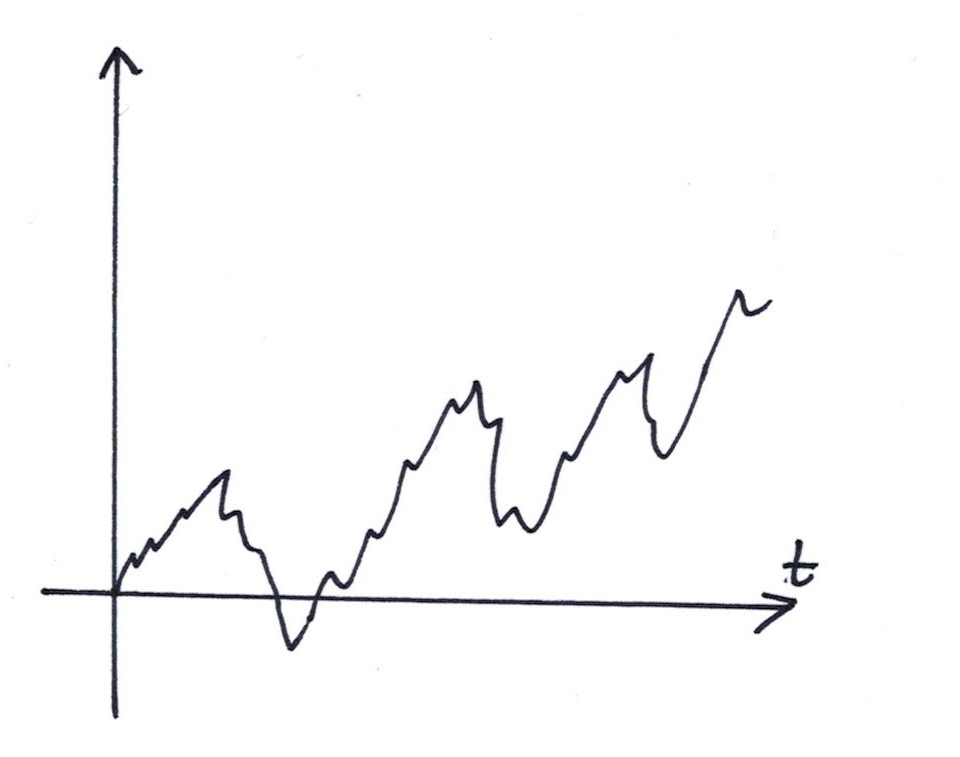
\includegraphics[width=0.5\linewidth]{04_lecture}
\end{figure}


Упражнение 1

\parindent=1cm

$X_t= - W_t$

Является ли $X_t$ винеровским процессом?

Естественная фильтрация: $\mathcal{F}_t=\sigma((Y_s))_{s\le t}$;

Проверим свойства винеровского процесса.

1) Х(0)=0;

2) Р(траектория $X_t$ непрерывна)=1;

3) $X_t-X_s$не зависит от $\mathcal{F}_s$;

4) $X_t-X_s \sim N(0;t-s)$;

5) $X_t$ измерим относительно  $\mathcal{F}_t$

Упражнение 2

\parindent=1cm

$Y_t=W_{8+t}-W_8$

Является ли $Y_t$ винеровским процессом?

Естественная фильтрация: $\mathcal{F}_t=\sigma((Y_S))_{s\le t}$;

Проверим свойства винеровского процесса.

1) Y$(0)=0$;

2) Р(траектория $Y_t$ непрерывна)=1;

3) $Y_t-Y_s=W_{8+t} - W_8-(W_{8+s} - W_8)=W_{8+t}-W_{8+s}$;

$\mathcal{H}_t=\sigma((W_s))_{s\le t}$

$\mathcal{F}_t=\sigma((Y_s))_{s\le t}=\sigma(W_{8+t}-W_8)_{s\le t}$

$\mathcal{F}_s\subseteq \mathcal{F}_{8+s}$

Сигма-алгебра $\mathcal{F}_{8+s}$ меньше, чем сигма-алгебра $\mathcal{F}_s$

4) $Y_t-Y_s=W_{8+t} - W_8-(W_{8+s} - W_8)=W_{8+t}-W_8-W_{8+s}+W_8 \sim N(0,t-s)$;

5) $Y_t$ измерим относительно $\mathcal{F}_t$


\section*{Независимоть величин}

Случайные величины А и В независимы, если $p(A\cap B)=p(A)\cdot p(B)$;

Независимость сигма-алгебр $\mathcal{F}$ и $\mathcal{H}$

$\forall$F$\in$\mathcal{F} и $\forall$H$\in$\mathcal{H}$

$p(F\cap H)=p(F)\cdot p(H)$;

Независимость случайной величины Х и сигма-алгебры $\mathcal{F}$:

${(X\le t)}$ и $\mathcal{F}$ - независимы;

$X=\sigma({x\le t}) $и $\mathcal{F}$ независимы;

\section*{Масштабирование}

$Z_t=\alpha W_2_t$

$F_t=\sigma((Z_s))_{s\le t$};

Найти $\alpha$ такое, чтобы $Z_t$ был Винеровским процессом.

Проверим свойства:

1) Z(0)=0;

2) Р(траектория $Z_t$ непрерывна)=1;

3) $Z_t-Z_s$ не зависит от $\mathcal{F}_s$ (независимость от прошлого);

4) Нормальность: $Z_t-Z_s= \alpha (W_{2t} - W_{2s}) \sim N(0;2t-2s)$; (Цель: $Z_t-Z_s \sim N(0;t-s))$;

$\alpha = \frac{1}{\sqrt{2}}$;

5) $X_t$ измерим относительно $\mathcal{F}_t$

Смысл свойства: сжатие по горизонтали в 2 раза, по вертикали в $\sqrt{2}$ раз.

\section*{Инверсия}

\begin{equation*}
R_t =
 \begin{cases}
   1, &\text{при $t=0$}\\
   f(t)\cdot W_\frac{1}{t}, &\text{при $t>0$}
 \end{cases}
\end{equation*}

Найдите $f(t)$ такую, что $R_t$ - Винеровский процесс

1) R(0)=0;

2) Траектория непрерывна;

$f(0)=0$;

$f(t)$ непрерывна;

3) Нормальность распределения

$R_t\sim N (0;t)$

$R_t-R_s \sim N (0;t-s)$

$f(t)\cdot W_\frac{1}{t} \sim N (0;\frac{1}{t})$

$var(f(t)\cdot W_\frac{1}{t})=f^2(t)\cdot \frac{1}{t}=t$

$f^2(t)=t^2$

f(t)=t

4) Независимость от прошлого;

5) $R_t$ измерим относительно $\mathcal{F}_t$

Геометрическое понимание свойства: инвертирует всю историю и упаковывает ее в интервал [0;1];

$R_1=W_1$

$R_2=2W_\frac{1}{2}$

$R_\frac{1}{2}=\frac{1}{2}W_2$

Упражнение

$E(W_4|W_7)=\frac{4}{7}W_7$

Применим инверсию

$W_4=4R_\frac{1}{4}$

$W_7=7R_\frac{1}{7}$

$E(4R_\frac{1}{4}|7R_\frac{1}{7})=4E(R_\frac{1}{4}|7R_\frac{1}{7})=4R_\frac{1}{7}=\frac{4}{7}W_7$

$E(4R_\frac{1}{4}|7R_\frac{1}{7})$ - В данном случае мы можем не обращать внимание на семерку внутри условия. Зная величину, умноженную на 7, мы можем вычислить значение самой величины. Например, нам не важно, в каких единицах измерени мы знаем темпиратуру воздуха: мы понимаем истинное значение и в градусах Цельсия, и в градусах Фаренгейта.

\parindent=2cm

Рассмотрим следующий пример:

\parindent=2cm

Сравним диспрерсии: $var(W_3|W_7)$ и $var(W_6|W_7)$.
Какая дисперсия будет больше?
Ближе к концу интервала дисперсия будет ниже ($var(W_6|W_7)$).
Максимальная дисперсия: $var(W_3_,_5|W_6)$ (середина интервала).

\begin{figure}[h!]
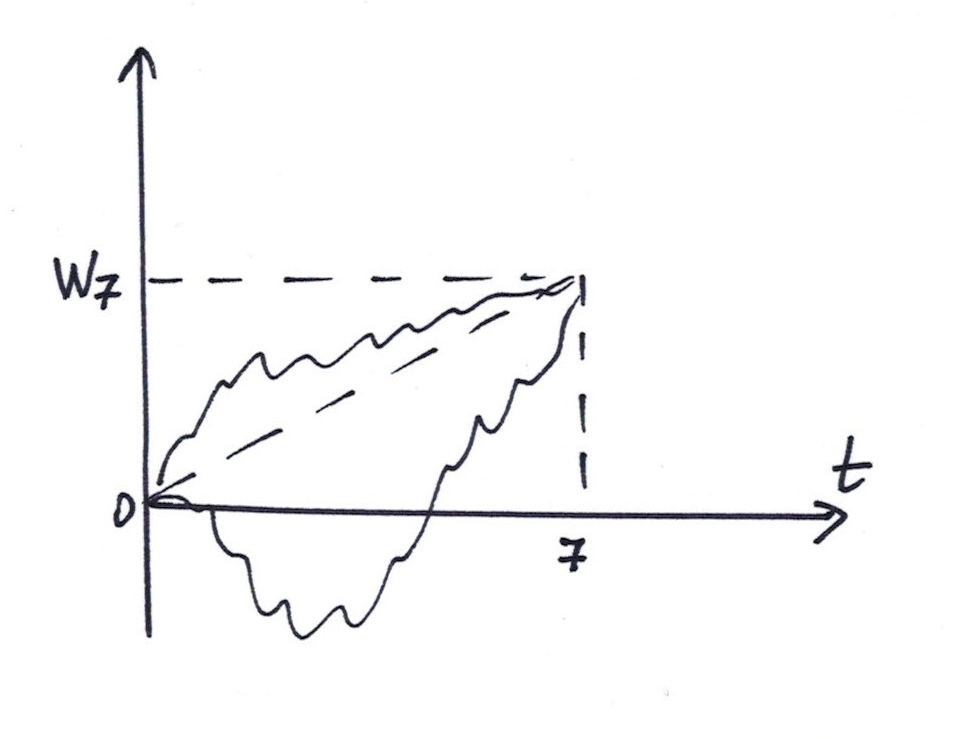
\includegraphics[width=0.5\linewidth]{04_lecture1}
\end{figure}

Мы знаем, что в нуле значение было, нулевым, а также знаем значение в конце. Точность в середине интервала меньше (выше дисперсия).

\section*{Стохастический интергал}

$$\int_{a}^{b} A_t dB_t$$ - прибыль инвестора за период времени от a до b;

$B_t$ - цена акции

$A_t$ - количество акций

Пример:

$\int_{0}^{3} 8 dt=8 t | _0^3=24$

Изначальное богатство: $8\cdot0$

Конечное богатство: $8\cdot3$

Прибыль: конечное богатство-начальное богатство = 24.

Упражнение 1

\parindent=1cm


$W_t$ - Винеровский процесс;

\begin{equation*}
X_t =
 \begin{cases}
   7, &\text{при $t \in [0;2]$}\\
   W_2, &\text{при $t\ge2$}
 \end{cases}
\end{equation*}

$$\int_{0}^{10} X_t dW_t$$

До второго момента:

$$\int_{0}^{2} X_t dW_t$$

Стохастическая величина: изначальное богатство: 7 акций по $W_0$ ($W_0=0$);

Держали до второго момента, потом докупили или продали.

Докупили ($W_2-7$) по цене $W_2$, потратили на это $W_2\cdot (W_2-7)$.

Десятый момент времени: Конечное богатство = $W_2\cdot W_{10}$;

Прибыль: Конечное богатство - Начальное богатство - Расходы на покупку.

$I=W_2\cdot W_{10}-7\cdot 0-W_2\cdot (W_2-7)=W_2\cdot W_{10}-W_2^2+7W_2$.

$E(W_2\cdot W_{10})=2$;

$E(W_2^2)=2$;

$E(7W_2)=0$;

$E(I)=0$.

Упражнение 2

\parindent=1cm


Пусть $X_1;X_2;X_3...\to X$;

1) $X_1;X_2;X_3...X \in L^2$;

$E(X_1^2)<\infty$;

$E(X_L^2)<\infty$;

Множество случайных величин, у которых конечное ожидание квадрата.

2) $E((X_i-X)^2) \to 0$

$X_1 \sim N (5;1)$;

$X_2 \sim N (5;\frac{1}{2})$;

$X_3 \sim N (5;\frac{1}{3})$;


$X_n \sim N (5;\frac{1}{n})$;

Сходится ли $X_n$ к чему-то?

Догадка: $X_n$ сходится к 5.

Проверка по определению:

$E((X_n-5)^2) = var (X_n)$ =$\frac{1}{n} \to 0.

Доказали: сходится к константе 5.

Упражнение на дом:

$W_t$ - Винеровский процесс;

$X_1=W_\frac{1}{n}-W_0$;

$X_2=W_\frac{2}{n}-W_\frac{1}{n}$;

Найти: $\sum\limits_{i=1}^n X_i^2  \to$ ? (в L2)




\end{document}
